\vspace{-0.45cm}

\section{Results} \label{sec:results}
    \begin{figure}
        \vspace{-0.5cm}
        
        \centering
        
        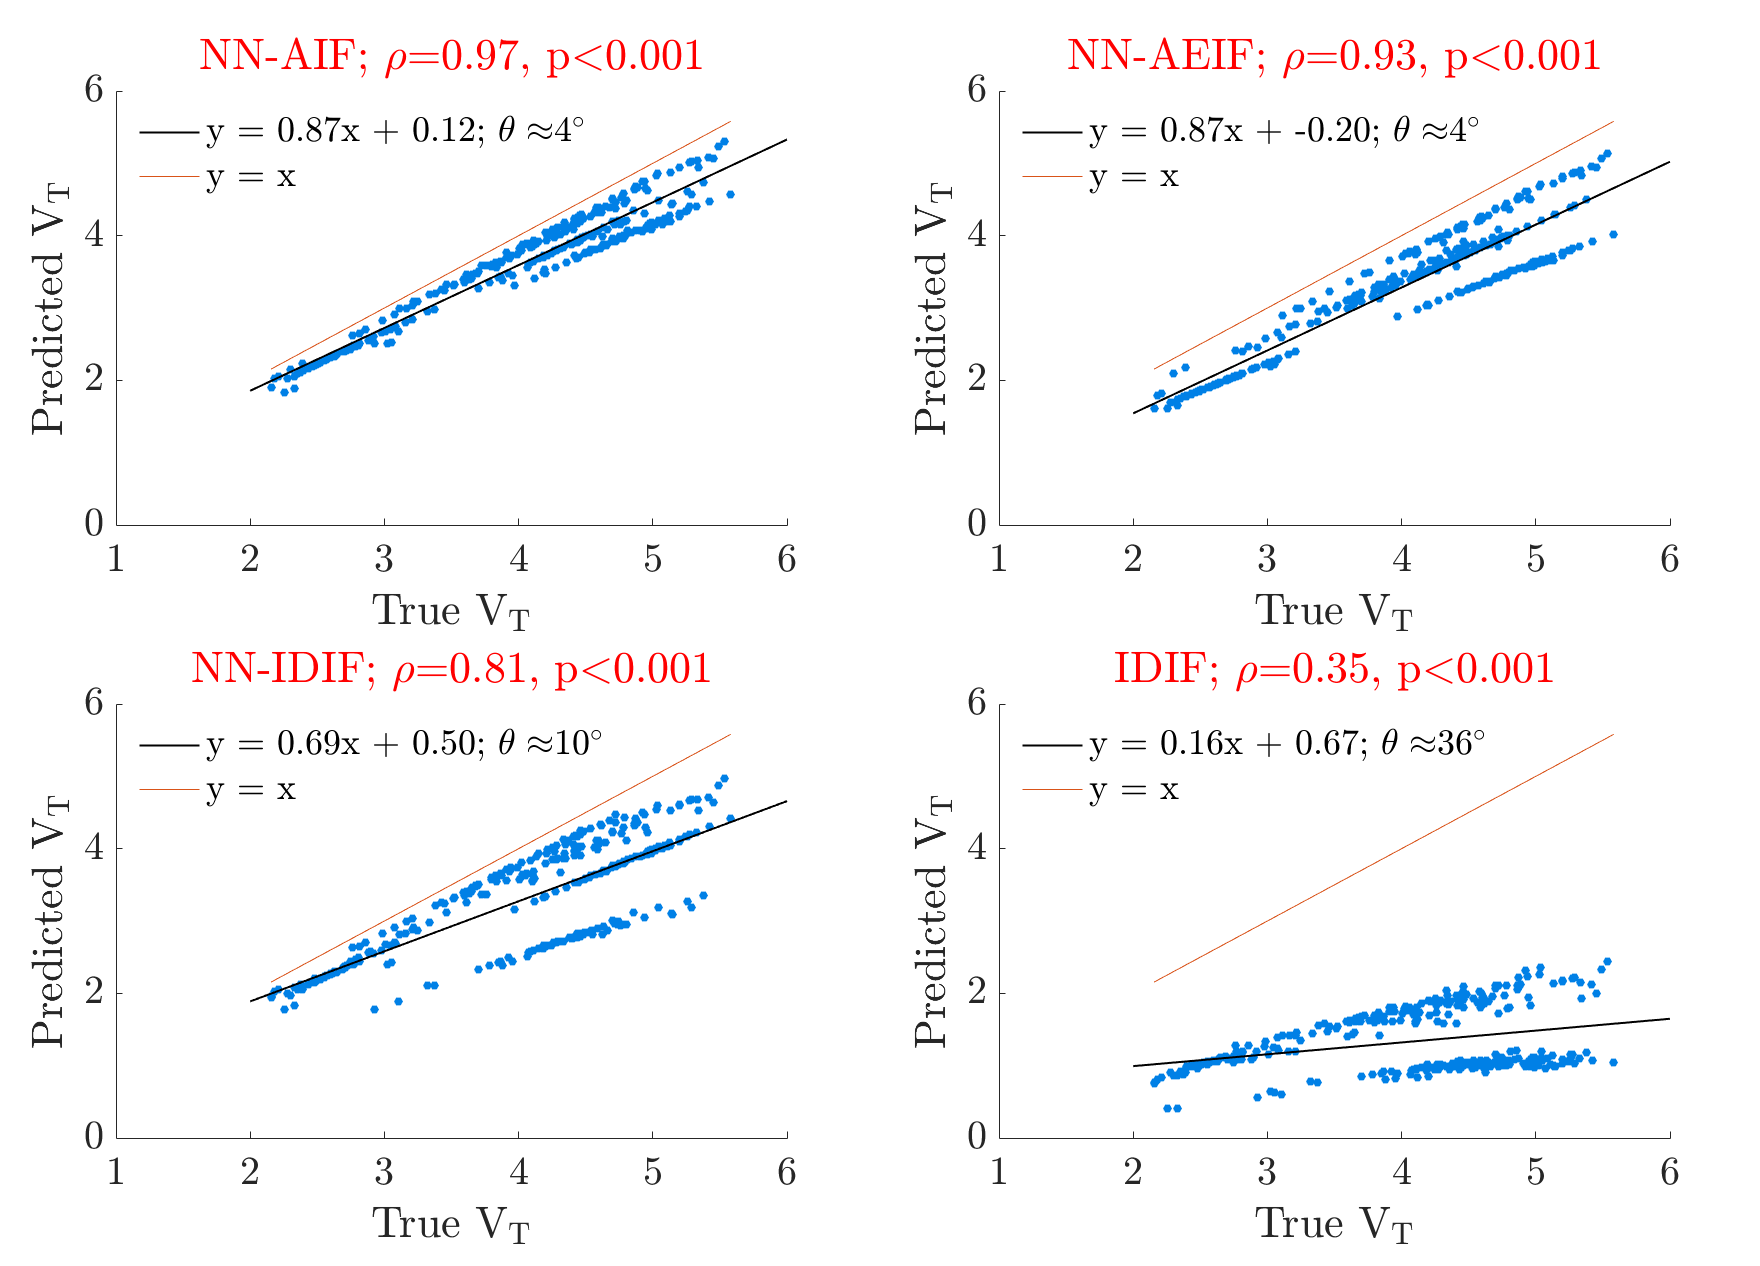
\includegraphics[width=1.0\linewidth]{Figures/correlation.png}
        
        \vspace{-0.25cm}
        
        \captionsetup{singlelinecheck=false, justification=centering}
        \caption{
            \scriptsize
            Predicted $V_{\mathrm{T}} \in \mathbb{R}^{r \times s}$ in the test-set subjects, with $r = 69$ and $s=5$ estimated with the four candidate signals, correlated to the True \gls{VT} (obtained with TRUE-\gls{AIF}). Please note that for the \gls{NN}-based methods, the displayed \glspl{VT} was averaged over all multiple realisations.
        }
        
        \label{fig:correlation}
        
       % \vspace{-0.5cm}
   \end{figure}

    
   \Fref{fig:correlation} reports the correlation analyses between the predicted \gls{VT} values (obtained by the four candidate methods) and the true \gls{VT}. For all methods, predicted \gls{VT} values positively correlate with true \gls{VT}, with \gls{NN}-\gls{AIF} and \gls{IDIF} showing the highest and the lowest Pearson correlation coefficient ($\rho$), as well as the smallest and largest angular distance to the identity line respectively: $\rho = 0.97 \; \& \;  \theta \approx 4^{\circ}$ vs $\rho = 0.35 \; \&  \; \theta \approx 36^{\circ}$. Overall, \gls{NN}-\gls{AE}\gls{IF} slightly outperforms \gls{NN}-\gls{IDIF} in terms of Pearson correlation coefficient and angular distance: $\rho = 0.93 \; \& \; \theta  \approx 4^{\circ}$ vs $\rho = 0.81 \; \&  \; \theta \approx 10^{\circ}$.

    With regard to the variance analysis, \gls{NN}-\gls{AE}\gls{IF} outperforms both \gls{NN}-\gls{AIF} and \gls{NN}-\gls{IDIF}, showing the lowest \gls{CV}, while \gls{NN}-\gls{AIF} and \gls{NN}-\gls{IDIF} do not differ in terms of \gls{CV} values (p$>0.05$).
